%
% Name: Parallel and Scientific Computing Coursework 2
% Author: Donald Whyte (sc10dw@leeds.ac.uk)
%

\documentclass{article}

% Make subsections use alphabet indices and not numeric indices
\renewcommand{\thesubsection}{\thesection.\alph{subsection}}

\usepackage[margin=3cm]{geometry} % easy page formatting
	
\usepackage{datetime} % up-to-date, automatically generated times
\usepackage{amsfonts}
\usepackage{amsthm}
\usepackage{amsmath}
\usepackage{graphicx}
\usepackage{float}
\usepackage{color}
	\definecolor{mygreen}{rgb}{0,0.6,0}
	\definecolor{mygray}{rgb}{0.5,0.5,0.5}
	\definecolor{mymauve}{rgb}{0.58,0,0.82}
\usepackage{listings}
\lstset{ %
  backgroundcolor=\color{white},   % choose the background color; you must add \usepackage{color} or \usepackage{xcolor}
  basicstyle=\footnotesize,        % the size of the fonts that are used for the code
  breakatwhitespace=false,         % sets if automatic breaks should only happen at whitespace
  breaklines=true,                 % sets automatic line breaking
  captionpos=b,                    % sets the caption-position to bottom
  commentstyle=\color{mygreen},    % comment style
  deletekeywords={...},            % if you want to delete keywords from the given language
  escapeinside={\%*}{*)},          % if you want to add LaTeX within your code
  extendedchars=true,              % lets you use non-ASCII characters; for 8-bits encodings only, does not work with UTF-8
  frame=single,                    % adds a frame around the code
  keepspaces=true,                 % keeps spaces in text, useful for keeping indentation of code (possibly needs columns=flexible)
  keywordstyle=\color{blue},       % keyword style
  language=Octave,                 % the language of the code
  morekeywords={*,...},            % if you want to add more keywords to the set
  numbers=left,                    % where to put the line-numbers; possible values are (none, left, right)
  numbersep=5pt,                   % how far the line-numbers are from the code
  numberstyle=\tiny\color{mygray}, % the style that is used for the line-numbers
  rulecolor=\color{black},         % if not set, the frame-color may be changed on line-breaks within not-black text (e.g. comments (green here))
  showspaces=false,                % show spaces everywhere adding particular underscores; it overrides 'showstringspaces'
  showstringspaces=false,          % underline spaces within strings only
  showtabs=false,                  % show tabs within strings adding particular underscores
  stepnumber=2,                    % the step between two line-numbers. If it's 1, each line will be numbered
  stringstyle=\color{mymauve},     % string literal style
  tabsize=2,                       % sets default tabsize to 2 spaces
  title=\lstname                   % show the filename of files included with \lstinputlisting; also try caption instead of title
}	

\title{Parallel and Scientific Computing \\ Coursework Two}
\author{Donald Whyte (sc10dw@leeds.ac.uk)}
\date{\today}

\begin{document}

\maketitle

\tableofcontents

\pagebreak

\section{Performance as Problem Size Grows}

The exact solution to the problem has been changed to $e^{3y}cos{3x}$, with a convergence tolerance of $10^{-12} = 0.000000000001$. The Laplace solver with Jacobi iteration was run on this problem using various problem sizes. The error of the approximated solutions for each of these problem sizes is given in Table \ref{tab:problem_size_growth}. Figure \ref{fig:problem_size_growth} shows a logarithmic plot of the problem size against the magnitude of the error. Notice how this plot is a straight line, going downwards as $N$ is increases.

This matches the values in Table \ref{tab:problem_size_growth}. Increasing $N$ decreases the magnitude of the error. Every time the problem size is \textbf{doubled} (interval is \textbf{halved}), the error is roughly \textbf{quartered}.

This means the error is proportional to the interval size. That is, $Error \in O(dx^2)$ where $Error$ is the error of the final solution and $dx$ is the interval size ("spacial" step) being used.

\begin{table}
	\centering
	\begin{tabular}{|l|l|}
	\hline
	\textbf{Problem Size (\textit{N})} & \textbf{Error} \\
	\hline
	8 & 2.59991e+01 \\
	16 & 6.90990e+00 \\
	32 & 1.87038e+00 \\
	64 & 4.76563e-01 \\
	128 & 1.19343e-01 \\
	256 & 2.98689e-02 \\
	512 & 7.46826e-03 \\
	\hline
	\end{tabular}
	\caption{Contains the error of the final solution produce by heat\_rows.c for different approximation intervals and a convergence tolerance of $10^{-12}$}
	\label{tab:problem_size_growth}
\end{table}

\begin{figure}
	\centering
	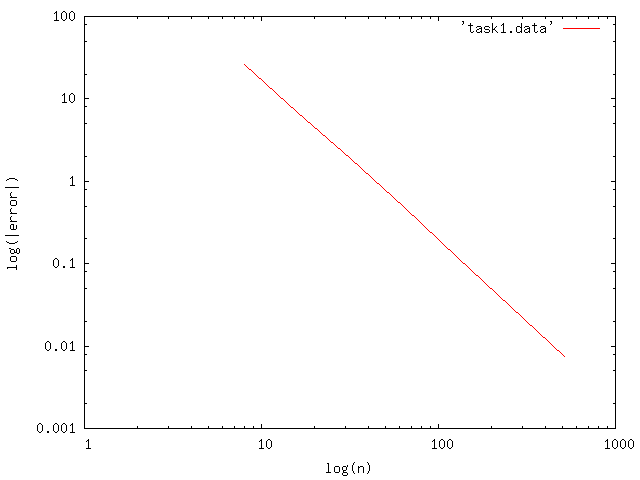
\includegraphics[width=0.8\textwidth]{task1/task1_plot.png}
	\caption{Logarithmic plot illustrating how error changes as approximation as problem size increases}
	\label{fig:problem_size_growth}
\end{figure}

\section{Larger Convergence Tolerance and its Effects}

The same experiences were performed as the ones in section 1, except with a convergence tolerance of $10^{-5} = 0.00001$. Table \ref{tab:larger_convergence_tolerance} and Figure \ref{fig:larger_convergence_tolerance} show the errors with different problem/interval sizes and a logarithmic plot of problem size against error respectively.

Initially, the behaviour of the error appears similar to when a convergence tolerance of $10^{-5}$ is used. Halving the interval size by doubling $N$ both roughly quarters the error repeatedly, until $N = 128$ is reached.

At that point, when $128$ is doubled to $256$, the error slightly increases. Doubling again to $512$ makes the error four times as large. This increase in error after $128$ is illustrated in Figure \ref{fig:larger_convergence_tolerance}. This shows that as you reduce the interval size, the error in the found solution starts to increase after a certain point. Exactly when the error starts increasing depends on what convergence tolerance is used.

The reason for this is larger problem sizes mean smaller interval sizes. This typically increases the accuracy of the found solution, but it means that \textbf{smaller changes per iteration} are inevitable. If the convergence tolerance is quite large, then these small changes will cause the algorithm to think it has converged to a solution and terminate. At that point, the current iteration is used as the solution, which may have a larger error because it has stopped prematurely.

\begin{table}
	\centering
	\begin{tabular}{|l|l|}
	\hline
	\textbf{Problem Size (\textit{N})} & \textbf{Error} \\
	\hline		
	8 & 2.59991e+01 \\
	16 & 6.90983e+00 \\
	32 & 1.87012e+00 \\
	64 & 4.75122e-01 \\
	128 & 1.13469e-01 \\
	256 & 1.29022e-01 \\
	512 & 4.44284e-01 \\
	\hline
	\end{tabular}
	\caption{Contains the error of the final solution produce by heat\_rows.c for different approximation intervals and a convergence tolerance of $10^{-5}$}
	\label{tab:larger_convergence_tolerance}
\end{table}

\begin{figure}
	\centering
	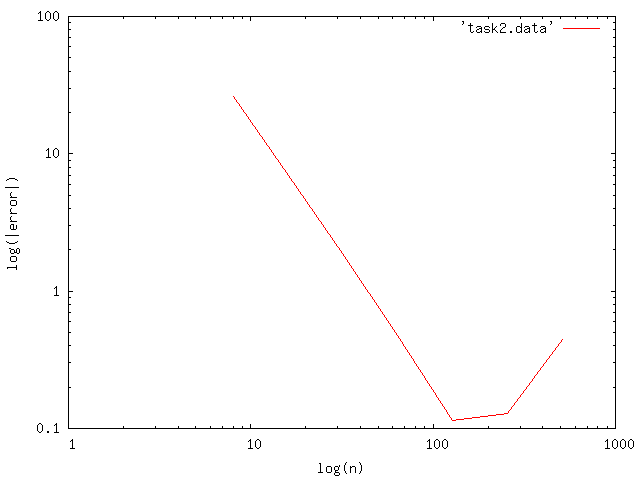
\includegraphics[width=0.8\textwidth]{task2/task2_plot.png}
	\caption{Logarithmic plot illustrating how error changes as approximation problem size increases}
	\label{fig:larger_convergence_tolerance}
\end{figure}

\section{Scalability of Row Decomposition}

\textbf{heat\_rows.c} was modified such that it always runs for exactly 8000 iterations. The execution times of Jacobi iteration with row decomposition for different problem sizes and number of processes were recorded. These times are shown in Table \ref{tab:row_decomp_scalability}.

For each problem size, the execution time to perform the 8000 iterations decreases as you increase the number of processes being used, \textbf{until} a certain number of processes is reached. At that number, adding any more processors \textbf{increases execution time}.

I suspect the reason for this is that any potential speedup achieved by parallelising the solver is \textbf{dominated} by the increased communication costs introduced when adding more processors. 

This is supported by the fact that the number of processors it takes to make the solver run slower increases as the problem size increases. This is because the speedup gained by parallelising for large values of $N$ dominates the time to takes to perform the extra communication. With small values of $N$, the execution time is reduced less, meaning the time spent with inter-process communication (which is the \textit{same} as it is for large values $N$) is larger than the reduction in time. Therefore, the final execution time for small problem sizes will actually be \textit{longer} than solving the problem with a single processor.

The reduction in also illustrated in Figure \ref{fig:row_decomposition_speedup_factors} and \ref{fig:row_decomposition_efficiency_factors}, which plot number of processors against the solver's \textbf{speedup} and \textbf{efficiency} factors respectively (for varying problem sizes). Notice how the speedup achieved by parallelising the solver drops off for each problem size, with the speedup of smaller problem sizes dropping off earlier with less processors.

The efficiency also shows this property; the overall efficiency of this implementation of parallel Jacobi steadily reduces as you increase the number of processors, with larger problem sizes dropping at much slower rates on average.

\paragraph{\textbf{NOTE:}} There are some fluctuations in the results (e.g. speedup and efficiency of $N = 961$). This is most likely due to spikes in use of the machines in the MPD ring. That said, the speedup and efficiency factor plots still show the overall relation between problem size and number of processes, so it shouldn't cause too much of an issue.

\begin{table}
	\centering
	\begin{tabular}{|l|l|l|}
	\hline
	\textbf{Problem Size (\textit{N})} & \textbf{\# Processors}  & \textbf{Execution Time (seconds)} \\ 
	\hline
	61 & 1 & 1.51095e-01 \\
	61 & 2 & 1.06213e-01 \\	
	61 & 4 & 2.52394e-01 \\	
	61 & 8 & 5.70459e+00 \\	
	61 & 16 & 9.74602e+00 \\	
	\hline
	121 & 1 & 7.06480e-01 \\
	121 & 2 & 4.10898e-01 \\
	121 & 4 & 3.53546e-01 \\
	121 & 8 & 5.35226e+00 \\
	121 & 16 & 1.07147e+01 \\
	\hline	
	241 & 1 & 2.50098e+00 \\
	241 & 2 & 1.46303e+00 \\
	241 & 4 & 1.03135e+00 \\
	241 & 8 & 7.08373e+00 \\
	241 & 16 & 1.52967e+01 \\ 
	\hline	
	481 & 1 & 1.51405e+01 \\
	481 & 2 & 8.39778e+00 \\ 
	481 & 4 & 4.23518e+00 \\
	481 & 8 & 8.64512e+00 \\
	481 & 16 & 1.64684e+01 \\
	\hline	
	961 & 1 & 5.34672e+01 \\ 
	961 & 2 & 3.43274e+01 \\
	961 & 4 & 2.46849e+01 \\
	961 & 8 & 1.53521e+01 \\ 
	961 & 16 & 2.22045e+01 \\
	\hline	
	1921 & 1 & 1.90737e+02 \\
	1921 & 2 & 1.35852e+02 \\
	1921 & 4 & 9.96819e+01 \\
	1921 & 8 & 5.21617e+01 \\
	1921 & 16 & 3.42827e+01 \\
	\hline
	\end{tabular}
	\caption{Table illustrating how the problem size and number of processes used affects runtime when using row decomposition}
	\label{tab:row_decomp_scalability}
\end{table}

\begin{figure}
	\centering
	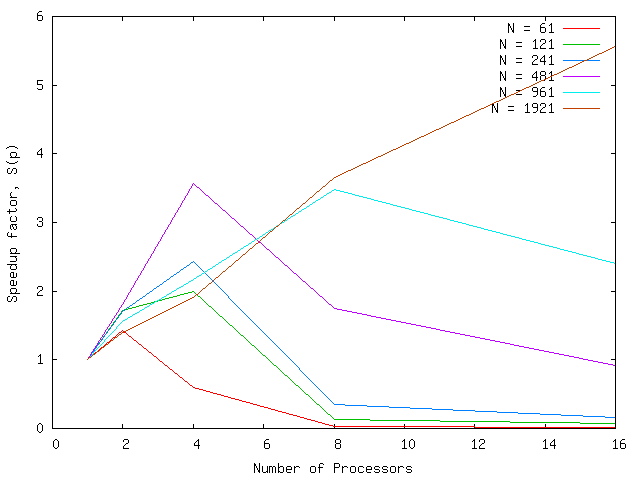
\includegraphics[width=0.8\textwidth]{task3/task3_row_speedups.png}
	\caption{Speedup achieved by parallelising the Laplace solver using row (strip) decomposition for different problem sizes}
	\label{fig:row_decomposition_speedup_factors}
\end{figure}

\begin{figure}
	\centering
	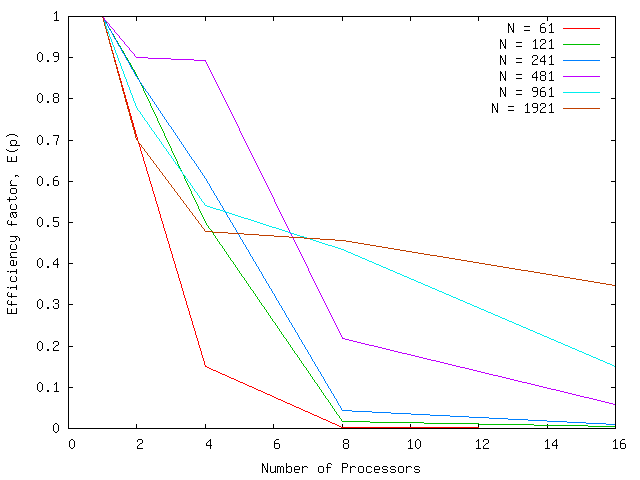
\includegraphics[width=0.8\textwidth]{task3/task3_row_efficiencies.png}
	\caption{Efficiency of parallel Laplace solver using row (strip) decomposition for different problem sizes}
	\label{fig:row_decomposition_efficiency_factors}
\end{figure}


\section{Scalability of Block Decomposition}

\textbf{heat\_blocks.c} was modified in the same way as \textbf{heat\_rows.c} in section 3. The execution times of Jacobi iteration with block decomposition for different problem sizes and number of processes were recorded and placed in Table \ref{tab:block_decomp_scalability}. Speedup and efficiency factor plots are shown in Figures \ref{fig:block_decomposition_speedup_factors} and \ref{fig:block_decomposition_efficiency_factors}.

Like strip decomposition, the execution time to perform the 8000 iterations decreases as you increase the number of processes being used \textbf{until} a certain number of processes is reached. At that number, adding any more processors \textbf{increases execution time}.

\subsection{More Scalable Partition Strategy}

So which partition strategy scales better as the number of processors is increased? Strip or block decomposition? Comparing the runtimes directly from Tables \ref{tab:row_decomp_scalability} and  \ref{tab:block_decomp_scalability}, block decomposition looks to be the better solution, as its execution times are consistently smaller than strip decomposition's, regardless of problem size.

However, if we compare the speedup and efficiency factors of the two strategies strip decomposition looks as if it would scale better as the number of processors is increased. The speedup gained by adding more processors is reduced slower with strip decomposition than block decomposition. In fact, Figures \ref{fig:row_decomposition_speedup_factors} and \ref{fig:block_decomposition_speedup_factors} show that the speedup with strip decomposition is still increasing when $N = 1921$ with 16 processors, whereas it has already started to decrease with block decomposition.

The same applies to the efficiency. The efficiency factor appears to start decreasing earlier with strip decomposition, but the rate at which efficiency is reduced is much slower. With $N = 1921$ and 16 processors, $E(p) \approx 0.35$ for strip decomposition and $E(p) \approx 0.19$ for block decomposition. 

Therefore, I would conclude that strip decomposition provides better scalability for the Laplace solver.

\subsection{Relation to Theoretical Parallel Time Complexity Analysis}

This contradicts the theoretical parallel time complexity analysis described in lectures. In that, block decomposition appeared to provide better scalability, based on the speedup factor plots shown. However, plots based on real runtime information appear to suggest that strip decomposition provides better overall scalability/efficiency.

In the theoretical analysis, the communications overhead with block decomposition may have been greatly underestimated in the theoretical analysis, or perhaps that the actual algorithm simply has a faster implementation for row decomposition. Processing, memory access and communication times all have an impact on performance,and they all vary based on the platform, the operating system and other processes running on the same machines. That is, the environment the experiments were run in could have been a factor in the produced plots too.

In practice, there is always a point at which adding more processes introduces so much communications overhead such that it dominates any speedup gained by parallelising the problem (as discussed in section 3). 

\begin{table}
	\centering
	\begin{tabular}{|l|l|l|}
	\hline
	\textbf{Problem Size (\textit{N})} & \textbf{\# Processors} & \textbf{Execution Time (seconds)} \\ 
	\hline
	61 & 1 & 1.08981e-01 \\
	61 & 4 & 7.82480e-02 \\
	61 & 9 & 6.11493e+00 \\
	61 & 16 & 6.73178e+00 \\
	\hline	
	121 & 1 & 3.38402e-01 \\
	121 & 4 & 1.77012e-01 \\
	121 & 9 & 7.14676e+00 \\
	121 & 16 & 8.37292e+00 \\
	\hline	
	241 & 1 & 1.21609e+00 \\
	241 & 4 & 4.80048e-01 \\
	241 & 9 & 7.11296e+00 \\
	241 & 16 & 1.07243e+01 \\
	\hline	
	481 & 1 & 4.50174e+00 \\
	481 & 4 & 1.48817e+00 \\
	481 & 9 & 1.11971e+01 \\
	481 & 16 & 1.39045e+01 \\
	\hline	
	961 & 1 & 2.08103e+01 \\
	961 & 4 & 1.20978e+01 \\
	961 & 9 & 1.65290e+01 \\
	961 & 16 & 1.93283e+01 \\
	\hline	
	1921 & 1 & 9.15544e+01 \\
	1921 & 4 & 5.14857e+01 \\
	1921 & 9 & 3.01908e+01 \\
	1921 & 16 & 3.20344e+01 \\
	\hline
	\end{tabular}
	\caption{Table illustrating how the problem size and number of processes used affects runtime when using block decomposition}
	\label{tab:block_decomp_scalability}
\end{table}

\begin{figure}
	\centering
	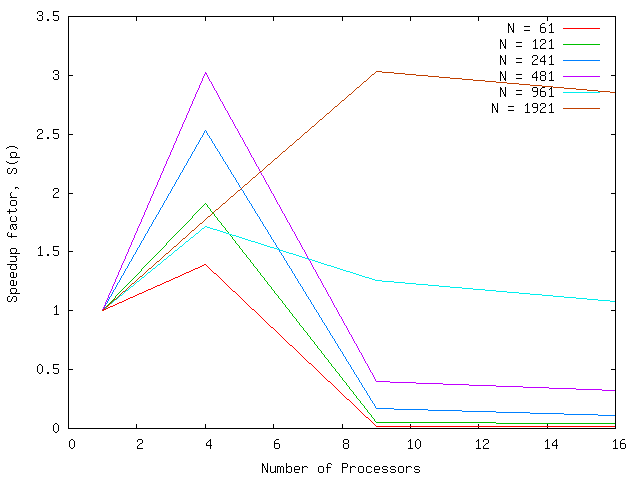
\includegraphics[width=0.8\textwidth]{task3/task3_block_speedups.png}
	\caption{Speedup achieved by parallelising the Laplace solver using block decomposition for different problem sizes}
	\label{fig:block_decomposition_speedup_factors}
\end{figure}

\begin{figure}
	\centering
	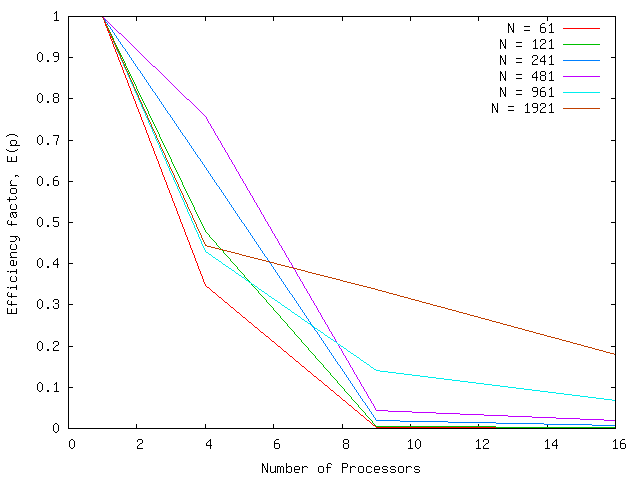
\includegraphics[width=0.8\textwidth]{task3/task3_block_efficiencies.png}
	\caption{Efficiency of parallel Laplace solver using block decomposition for different problem sizes}
	\label{fig:block_decomposition_efficiency_factors}
\end{figure}

\section{Jacobi and Gauss-Seidel Iteration}

\subsection{Lexicographic Gauss-Seidel on a Single Processor}

Lexicographic Gauss-Seidel iteration was implemented in the file \textbf{lexicographic\_gauss.c}. The number of iterations it took for algorithm to converge to the exact solution where $u = 1$ and $N = 241$, with different convergence tolerances of $10^{-12}$, were recorded.

These iteration counts are available in Table \ref{tab:jacobi_gauss_iteration_counts}, along with how many iterations to took the original Jacobi solver to be implemented.

As the convergence tolerance is increased, the number of iterations reached to converge to a solution is reduced for \textbf{both} Jacobi and Gauss-Seidel. When using the same convergence tolerance, Gauss-Seidel roughly takes \textbf{half} the number of iterations to converge to a solution as Jacobi. For example, when $Tol = 10^{-12}$, Jacobi takes $220567$ iterations whereas Gauss-Seidel takes $114365 \approx \frac{220567}{2}$ iterations. This is well-known property of Gauss-Seidel and generally holds true for most computational problems.

\subsection{Lexicographic Gauss-Seidel on Multiple Processors}

Table \ref{tab:jacobi_gauss_parallel_iteration_counts} shows how many iterations it to took for Jacobi and Lexicographic Gauss-Seidel to converge with $N = 241$ and a convergence tolerance of $10^{-12}$.

There is no change in the number of iterations required by Jacobi to converge from when it was run on a single processor. This is unsurprising, since adding more processors does not actually impact the computation in anyway.

The number of iterations required by Lexicographic Gauss-Seidel is still roughly half the number of iterations it takes for Jacobi to converge, however this property starts to weaken as you increase the number of processors.

Table \ref{tab:jacobi_gauss_parallel_iteration_counts} shows that the number of iterations for Gauss-Seidel increases steadily. I believe the reason for this is the order in which computations and communication is performed on each processor. The \textit{boundary} values each process contains depend on newly computed values from other processors. Since those new values (used for Gauss-Seidel iteration) are not received by a process until \textit{after} the whole iteration, the current iteration uses old values where new values should have been used, which slows the convergence.

In other words, as increase the number of processors, the more and more old values (from iteration $k$, not $k + 1$) are used for the computation. This causes the Gauss-Seidel algorithm to become closer and closer to Jacobi. If the number of processors was $(N - 1)$, then lexicographic Gauss-Seidel would essentially be Jacobi iteration, because each process would try and use its "new" values, but would actually be using values from the previous iteration $k$ (since the new values for iteration $k + 1$ have not been received from the other processors yet).

\begin{table}
	\centering
	\begin{tabular}{|c|c|c|}
		\hline
		\textbf{Algorithm} &
		\begin{tabular}{c}
			\textbf{Convergence} \\
			\textbf{Tolerance}
		\end{tabular}
		& \textbf{\# Iterations} \\
		\hline
		Jacobi & $10^{-12}$ & 220567 \\
		Gauss-Seidel & $10^{-12}$ & 114365 \\
		Jacobi & $10^{-10}$ & 166368 \\
		Gauss-Seidel & $10^{-10}$ & 87265 \\
		Jacobi & $10^{-8}$ & 112169 \\
		Gauss-Seidel & $10^{-8}$ & 60165 \\
		Jacobi & $10^{-6}$ & 57969 \\
		Gauss-Seidel & $10^{-6}$ & 33065 \\
		\hline
	\end{tabular}
	\caption{Shows how many iterations are required by the Jacobi and Gauss-Seidel algorithms to converge to a solution with a particular error tolerance}
	\label{tab:jacobi_gauss_iteration_counts}
\end{table}

\begin{table}
	\centering
	\begin{tabular}{|c|c|c|}
		\hline
		\textbf{Algorithm} & \textbf{\# Processors} & \textbf{\# Iterations} \\
		\hline
		Jacobi & $2$ & 220567 \\
		Jacobi & $3$ & 220567 \\
		Jacobi & $4$ & 220567 \\		
		Gauss-Seidel & $2$ & 116198 \\
		Gauss-Seidel & $3$ & 117053 \\
		Gauss-Seidel & $4$ & 117994 \\
		\hline
	\end{tabular}
	\caption{Shows how many iterations are required by the Jacobi and Gauss-Seidel algorithms to converge to a solution using a convergence tolerance of $10^{-12}$, when different numbers of processors are being used}
	\label{tab:jacobi_gauss_parallel_iteration_counts}
\end{table}

\section{Red-Black Gauss-Seidel Iteration}

\textbf{redblack\_gauss.c} contains a parallel implementation of red-black Gauss-Seidel iteration. Table \ref{tab:red_black_gauss_iteraton_counts} shows how many iterations it takes this algorithm to converge with different convergence tolerances, both on one and four processors. 

For one processor, red-black Gauss-Seidel iteration uses the same amount of iterations is the same as lexicographic Gauss-Seidel. Unlike the lexicographic algorithm however, the number of iterations red-black version uses does not increase as you increase the number of processors (as long as the number of processors $p$ makes $\frac{(N - 1)}{p}$ an even integer). In other words, red-black Gauss-Seidel scales to more processors and parallelises much better than lexicographic Gauss-Seidel.

Table \ref{tab:red_black_gauss_iteraton_counts} also contains iteration counts for when I ran the algorithm on a $p$ processors where $\frac{(N - 1)}{p}$ is not an even integer. In other words, when the work is not be evenly distributed among the processes (one will have less work than the others). The numbers I used were 7, 9 and 11. 

The key difference here is that the number of iterations required to converge \textit{increases slightly}, in a similar fashion to lexicographic Gauss-Seidel. This is due to the fact that there will be some processes where the first node on the first row is actually a \textit{black} node, but the processes itself will treat it as a red  node (because it's the first node of the array). This causes a mismatch on the latest values at the boundaries of some processes  (values from iteration $k$ used where values from $k + 1$ should be) , which affect the speed at which the algorithm converges.

\begin{table}
	\centering
	\begin{tabular}{|c|c|c|}
		\hline
		\textbf{\# Processors} &
		\begin{tabular}{c}
			\textbf{Convergence} \\
			\textbf{Tolerance}
		\end{tabular}
		& \textbf{\# Iterations} \\
		\hline
		$1$ & $10^{-12}$ & 114365 \\
		$1$ & $10^{-10}$ & 87265 \\
		$1$ & $10^{-8}$ & 60165 \\
		$1$ & $10^{-6}$ & 33065 \\
		\hline
		$4$ & $10^{-12}$ & 114365 \\
		$4$ & $10^{-10}$ & 87265 \\
		$4$ & $10^{-8}$ & 60165 \\
		$4$ & $10^{-6}$ & 33065 \\
		\hline
		$7$ & $10^{-12}$ & 114741 \\
		$9$ & $10^{-12}$ & 116152 \\
		$11$ & $10^{-12}$ & 114403 \\
		$7$ & $10^{-6}$ & 33159 \\
		$9$ & $10^{-6}$ & 33508 \\
		$11$ & $10^{-6}$ & 33077 \\
		\hline
	\end{tabular}
	\caption{How many iterations red-black Gauss-Seidel iteration requires with different convergence tolerances}
	\label{tab:red_black_gauss_iteraton_counts}
\end{table}

\section{Successive Over-Relaxation}

\textbf{sor.c} is a modification of \textbf{redblack\_gauss.c} which makes use of Successive Over-Relation. The relaxation parameter $\omega$ which produced the optimal number of iterations for the problem $u =  1, N = 241, Tol=10^{-12}$ was found.

Table \ref{tab:sor_relaxation_parameter_multiple_proc} shows the iteration counts for different values of $\omega$. Note that for some values $\omega$, particular very high values, SOR never converged and continuously fluctuated between two different values. These are marked appropriately in the table.
 $\omega =$ \textbf{1.98} produced the lowest number of iterations (1339).

\begin{table}
	\centering
	\begin{tabular}{|c|c|c|}
		\hline
		\textbf{$w$} & \textbf{\# Iterations} \\
		\hline
		0.9 & 138338 \\
		1.0 & 114365 \\
		1.1 & 94536 \\
		1.2 & 77831 \\
		1.3 & 63538 \\
		1.4 & 51143 \\
		1.5 & 40266 \\
		1.6 & 30615 \\
		1.7 & 21959 \\
		1.8 & 14102 \\
		1.9 & 6835 \\
		1.91 & 6128 \\
		1.92 & 5420 \\
		1.93 & 4711 \\
		1.94 & 3995 \\
		1.95 & 3267 \\
		1.96 & 2509 \\
		1.97 & 1653 \\
		\textbf{1.98} & \textbf{1339} \\
		1.99 & 2709 \\
		2.0 & $> 150000$ (does not converge) \\
		\hline
	\end{tabular}
	\caption{How relaxation parameter affects number of iterations when using a convergence tolerance of $10^{-12}$ on \textbf{four processors}}
	\label{tab:sor_relaxation_parameter_multiple_proc}
\end{table}

\section{Comparison of the Three Iterative Methods}

\subsection{Comparison on a Single Processor}

The runtimes of Jacobi, red-black Gauss-Seidel and red-black Successive Over-Relaxation when solving $u = 1, N = 241$ with a convergence tolerance of $10^{-12}$ have been recorded in Table \ref{tab:overall_runtimes}.

On a single processor, Jacobi and red-black Gauss-Seidel iteration have similar runtimes, with red-black Gauss-Seidel taking a little longer. While red-black Gauss-Seidel took half the iterations as Jacobi, each iteration takes more than twice as long as an one iteration of Jacobi (as shown in Table \ref{tab:overall_runtimes}). Therefore, there is no gain on speed with a single processor. Red-black Gauss-Seidel's iterations take longer than Jacobi's because there are two lots of communication per iteration and two passes through the array to update the red and black nodes separately.

A single iteration of red-black SOR takes a similar amount of time as red-black Gauss-Seidel. However, it runs significantly faster overall due to the massive reduction in iterations. On a single processor, red-black SOR is by far the fastest, being over $30$ times faster than the other two algorithms.

\subsection{Comparison on Multiple Processors}

On multiple processors, red-black Gauss-Seidel now outperforms Jacobi. This is because it now uses a low enough number of iterations that the extra cost per iteration (compared to Jacobi) does not outweigh the savings in time from less iterations. SOR still beats red-black Gauss-Seidel by a large margin, requiring less iterations and thus, less time, to converge.

By parallelising, the runtimes of each individual iteration has been reduced, but the \textit{relationship} between iteration runtimes for each algorithm remains the same. One iteration of red-black Gauss-Seidel still takes roughly double the time of a single iteration of Jacobi and red-black SOR still has a similar iteration runtime as red-black Gauss-Seidel.

\subsection{Shortest Runtime Achieved}

The shortest run-time I achieved with a convergence tolerance of $10^{-12}$ is 0.334205 seconds. This was from using red-black Successive Over-Relaxation (with $\omega = 1.98$ on four processors). This is approximately $\frac{34.22217}{0.334205} \approx 102$ times faster than running Jacobi iteration on a single processor.

\paragraph{\textbf{NOTE}: } If the number of processes used to execute SOR is increased to five processors, then the communications overhead of having more processors starts to dominate, making the overall runtime \textit{slower} than four processors. 

\begin{table}
	\centering
	\begin{tabular}{|l|l|l|l|l|}
		\hline
		\textbf{Algorithm} & \textbf{\# Processors} &
		\begin{tabular}{c}
			\textbf{Runtime} \\
			\textbf{(in seconds)}
		\end{tabular} &
		\textbf{\# Iterations} &
		\begin{tabular}{c}
			\textbf{Runtime} \\
			\textbf{per Iteration}
		\end{tabular} \\
		\hline
		Jacobi & 1 & 34.2217 & 220567 & 0.0001551533 \\
		Red-Black Gauss Seidel & 1 & 43.2007
 & 114365 & 0.00037774406 \\
		Red-Black SOR ($\omega = 1.98$)& 1 & 1.07561 & 1339 & 0.0008032935 \\
		Jacobi & 4 & 18.0577 & 220567 & 0.00008186945\\
		Red-Black Gauss Seidel & 4 & 12.2005
 & 114365 & 0.00010668036  \\
		Red-Black SOR ($\omega = 1.98$) & 4 & 0.334205
 & 1339 & 0.00024959297 \\		
		\hline
	\end{tabular}
	\caption{Runtime of different algorithms with varying number of processors for $u = 1, N = 241$ and a convergence tolerance of $10^{-12}$}
	\label{tab:overall_runtimes}
\end{table}

\section{Appendix}

\subsection{Task 1 Code Modifications} 

The original source code contains a function called exact(), which returns the exact solution at point $(x, y)$. To change the exact solution to $e^{3y}\cos{3x}$, the following code was used:

\begin{lstlisting}[language=C]
double exact( double x, double y )
{
  double solution;

  solution = exp(3 * y) * cos(3 * x);

  return (solution);
}
\end{lstlisting}

The convergence tolerance was set to $10^{-12}$ by changing the $Tol$ macro like so:
\begin{lstlisting}[language=C]
#define Tol 0.000000000001
\end{lstlisting}

\subsection{Task 3 Code Modifications} 

To fix the number of iterations for both \textbf{heat\_rows.c} and \textbf{heat\_blocks.c}, I defined a new constant:
\begin{lstlisting}[language=C]
#define MAX_ITER 8000
\end{lstlisting}

Then I changed the stopping criteria by changing the condition of the algorithm's while-loop:
\begin{lstlisting}[language=C]
while ( iter<MAX_ITER )
\end{lstlisting}

\subsection{Task 4 MPD Ring}

An MPD ring with the following machines were used to obtain runtimes for tasks 4 and 4.
\begin{itemize}
	\item cslin011
	\item cslin012
	\item cslin013
	\item cslin014
\end{itemize}
Four processes (i.e. four CPUs) were used for each machine, allowing for a maximum of 16 simultaneous processes.

\subsection{Task 5 Code Modifications} 

To implement lexicographic Gauss-Seidel, I simply modified the equation inside the \textbf{iteration()} function to use the newly updated values for the left and top neighbouring nodes:
\begin{lstlisting}[language=C]
new[i][j] = 0.25 * ( old[i+1][j] + new[i-1][j] + old[i][j+1] + new[i][j-1] );
\end{lstlisting}

\subsection{Task 6 Full Source Code -- redblack\_gauss.c}

\begin{lstlisting}[language=C,frame=single]
/*
 * Parallel implementation of 2D Laplace equation solver
 *   -- Jacobi iteration
 *   -- partitioning done by strips of rows
 *   -- non-constant boundary conditions specified
 *   -- exact solution compared with
 *
 * Code supplied by Peter Jimack and modified by Matthew Hubbard */

#include <stdlib.h>
#include <stdio.h>
#include <math.h>
#include <mpi.h>

/* Define parameter values */
#define N 241
#define Tol 0.000000000001
// 10^-5 = 0.00001
// 10^-6 = 0.000001
// 10^-8 = 0.00000001
// 10^-10 = 0.0000000001
// 10^-12 = 0.000000000001

/* Define the geometric bounds of the domain */
#define xmin -2.0
#define xmax  2.0
#define ymin -2.0
#define ymax  2.0

enum NodeType {
    NODE_TYPE_RED = 0,
    NODE_TYPE_BLACK
};


/* Allocate memory for a two-dimensional array (pointers to pointers) */
double **matrix( int m, int n )
{
  int i;
  double **ptr;

  ptr = (double **) calloc( m, sizeof(double *) );
  for ( i=0; i<m; i++ )
    ptr[i] = (double *) calloc( n, sizeof(double) );

  return (ptr);
}



/* Carry out a single Jacobi iteration on the specified range of mesh nodes */
double iteration( double **mesh, int first_row, int last_row, int first_col, int last_col, enum NodeType nodeType )
{
  double diff, maxdiff=0.0;
  int i, j;
  int isEven=0;
  double old=0.0;

  for ( i=first_row; i<=last_row; i++ )
    for ( j=first_col; j<=last_col; j++ ) {
      old = mesh[i][j];
      /* The red-black Gauss-Seidel update for node (i,j) */
      isEven = (i + j) % 2;
      if ((isEven && nodeType == NODE_TYPE_RED) ||
        (!isEven && nodeType == NODE_TYPE_BLACK)) {
          mesh[i][j] = 0.25 * ( mesh[i+1][j] + mesh[i-1][j] + mesh[i][j+1] + mesh[i][j-1] );
      }

      /* Update the max norm of  x^(k+1) - x^(k) */
      diff = mesh[i][j] - old;
      if ( diff<0 )
        diff = -diff;
      if ( maxdiff<diff )
        maxdiff = diff;
    }

  /* Return the max norm of  x^(k+1) - x^(k)  for the specified range of nodes */
  return (maxdiff);
}



/* Calculate the exact solution at point (x,y) */
double exact( double x, double y )
{
  double solution;

  solution = 1.0;

  return (solution);
}



/* Calculate the max norm error in the final approximation on the specified range of
 * mesh nodes                                                                        */
double final_error( double **mesh, int start_row, int nrows, int start_col, int ncols, double dx, double dy )
{
  double x, y, diff, maxerr=0.0;
  int i, j;

  for ( i=1; i<=nrows; i++ ) {
    for ( j=1; j<=ncols; j++ ) {
      /* Calculate the geometric coordinates of point (i,j) */
      x = xmin + dx * (double) (start_row+i-1);
      y = ymin + dy * (double) (start_col+j-1);

      /* Update the max norm of  approximate - exact */
      diff = mesh[i][j] - exact( x, y );
      if ( diff<0 )
        diff = -diff;
      if ( maxerr<diff )
        maxerr = diff;
    }
  }

  /* Return the max norm of  approximate - exact  for the specified range of nodes */
  return (maxerr);
}



/* Write the approximate solution out to a single data file from process 0
 *   -- the format is row-by-row                                           */
void write_file( int nid, double **mesh, int rowmin, int rowmax, int colmin, int colmax, int first_row, int first_col, int noprocs )
{
  double **full;
  double *send_buffer, *recv_buffer;
  int row, col, counter, i, j, ip;
  int imin, imax, jmin, jmax;
  int send_indices[4], recv_indices[4];
  int send_size, recv_size;
  FILE *fp;
  MPI_Status status;


  /* Fix local row and column indcies */
  imin = rowmin - first_row + 1;
  imax = rowmax - first_row + 1;
  jmin = colmin - first_col + 1;
  jmax = colmax - first_col + 1;


  if ( nid==0 ) {
    /* Allocate memory on process 0 to store the full solution */
    full = matrix( N+1, N+1 );

    /* Insert the solution values calculated on process 0 in to the full array */
    for ( row=rowmin, i=imin; row<rowmax+1; row++, i++ )
      for ( col=colmin, j=jmin; col<colmax+1; col++, j++ )
        full[row][col] = mesh[i][j];

    /* Receive solution values from the other processes and enter them in to the full array */
    for ( ip=1; ip<noprocs; ip++ ) {
      /* Receive the indices indicating the solution values calculated on process ip */
      MPI_Recv( &recv_indices[0], 4, MPI_INT, ip, 25, MPI_COMM_WORLD, &status );

      rowmin = recv_indices[0]; rowmax = recv_indices[1];
      colmin = recv_indices[2]; colmax = recv_indices[3];

      /* Calculate the number of solution values to be sent by process ip */
      recv_size   = (rowmax-rowmin+1)*(colmax-colmin+1);
      recv_buffer = (double *) calloc( recv_size, sizeof(double) );

      /* Receive the solution values calculated on process ip */
      MPI_Recv( &recv_buffer[0], recv_size, MPI_DOUBLE, ip, 15, MPI_COMM_WORLD, &status );

      /* Place the solution values in the message in to the full array, in order */
      counter = 0;
      for ( row=rowmin; row<rowmax+1; row++ )
        for ( col=colmin; col<colmax+1; col++ ) {
          full[row][col] = recv_buffer[counter];
          counter++;
        }

      free( recv_buffer );
    }

    /* Write out the full array to  heat_solution.dat  row by row */
    fp = fopen( "heat_solution.dat", "wt" );

    for ( row=0; row<N+1; row++ )
      for ( col=0; col<N+1; col++ )
        fprintf( fp, "%6d %6d %8.6f\n", row, col, full[row][col] );

    fclose( fp );

    free( full );
  }
  else {
    send_indices[0] = rowmin; send_indices[1] = rowmax;
    send_indices[2] = colmin; send_indices[3] = colmax;

    /* Send the indices indicating the solution values to be sent to process 0 */
    MPI_Send( &send_indices[0], 4, MPI_INT, 0, 25, MPI_COMM_WORLD );

    /* Calculate the number of solution values to be sent to process 0 */
    send_size   = (imax-imin+1)*(jmax-jmin+1);
    send_buffer = (double *) calloc( send_size, sizeof(double) );

    /* Place the solution values to be sent in to the message in a specific order */
    counter = 0;
    for ( i=imin; i<imax+1; i++ )
      for ( j=jmin; j<jmax+1; j++ ) {
        send_buffer[counter] = mesh[i][j];
        counter++;
      }

    /* Send the solution values calculated on this process to process 0 */
    MPI_Send( &send_buffer[0], send_size, MPI_DOUBLE, 0, 15, MPI_COMM_WORLD );

    free( send_buffer );
  }
}

void synchronise_nodes(double** nodeValues, int nrows, int ncols, int nid, int noprocs)
{
    MPI_Status status;
    if ( nid<noprocs-1 ) {
      MPI_Send( &nodeValues[nrows][1],   ncols, MPI_DOUBLE, nid+1, 10, MPI_COMM_WORLD );
      MPI_Recv( &nodeValues[nrows+1][1], ncols, MPI_DOUBLE, nid+1, 20, MPI_COMM_WORLD, &status  );
    }
    if ( nid>0 ) {
      MPI_Send( &nodeValues[1][1], ncols, MPI_DOUBLE, nid-1, 20, MPI_COMM_WORLD );
      MPI_Recv( &nodeValues[0][1], ncols, MPI_DOUBLE, nid-1, 10, MPI_COMM_WORLD, &status  );
    }
}


/* Main program */
int main( int argc, char **argv )
{
  double **mesh, **tmp;
  double diff, MaxDiff, MaxDiffG, MaxErr, MaxErrG;
  double dx, dy, x, y;
  double start_time=0.0, end_time=0.0;
  int first_row, nrows, first_col, ncols;
  int noprocs, nid, remainder, i, j, iter;
  int rowmin, rowmax, colmin, colmax;
  MPI_Status status;
  MPI_Request req_send10, req_send20, req_recv10, req_recv20;


  /* Initialise for MPI */
  MPI_Init( &argc, &argv );
  MPI_Comm_rank( MPI_COMM_WORLD, &nid );
  MPI_Comm_size( MPI_COMM_WORLD, &noprocs );


  /* Calculate the mesh size */
  dx = ( xmax - xmin ) / (double) N;
  dy = ( ymax - ymin ) / (double) N;


  /* Calculate the first row and the number of rows allocated to this process */
  first_row = 1;
  remainder = (N-1)%noprocs;
  nrows     = (N-1-remainder)/noprocs;
  /* Care is taken with any left over rows after dividing the number of rows by the number of
   * processes: they are allocated one-by-one to the first few processes to avoid having one
   * process taking much more work than all of the others                                     */
  for ( i=0; i<nid; i++ ) {
    if ( i<remainder )
      first_row = first_row + nrows + 1;
    else
      first_row = first_row + nrows;
  }
  if ( nid<remainder )
    nrows++;

  /* Calculate the first column and the number of columns allocated to this process */
  first_col = 1;
  ncols     = N-1;


  /* Allocate memory for the local work arrays */
  mesh = matrix( nrows+2, ncols+2 );


  if ( nid==0 )
    start_time = MPI_Wtime();


  /* Apply boundary conditions at the ymin and ymax boundaries */
  for ( i=0; i<=nrows+1; i++ ) {
    x = xmin + dx * (double) (first_row+i-1);
    y = ymin;
    mesh[i][0] = exact( x, y );
    y = ymax;
    mesh[i][ncols+1] = exact( x, y );
  }

  /* Apply boundary conditions at the xmin and xmax boundaries */
  if ( nid==0 )
    for ( j=1; j<=ncols; j++ ) {
      x = xmin;
      y = ymin + dy * (double) (first_col+j-1);
      mesh[0][j]     = exact( x, y );
    }
  if ( nid==noprocs-1 )
    for ( j=1; j<=ncols; j++ ) {
      x = xmax;
      y = ymin + dy * (double) (first_col+j-1);
      mesh[nrows+1][j] = exact( x, y );
    }

  // Just set so one iteration of the loop is guaranteed to fire
  MaxDiffG = Tol * 2;
  iter = 1;
  while ( MaxDiffG>Tol ) { /* The error estimate is still too large */
    MaxDiff = iteration(mesh, 1, nrows, 1, N-1, NODE_TYPE_RED);
    synchronise_nodes(mesh, nrows, ncols, nid, noprocs);
    diff = iteration(mesh, 1, nrows, 1, N-1, NODE_TYPE_BLACK);
    synchronise_nodes(mesh, nrows, ncols, nid, noprocs);
    if (diff > MaxDiff)
        MaxDiff = diff;

    /* Estimate the error for the complete update */
    MPI_Allreduce( &MaxDiff, &MaxDiffG, 1, MPI_DOUBLE, MPI_MAX, MPI_COMM_WORLD );

    /* Write out the error estimate every 1000 iterations */
    iter++;
    if ( nid==0 && iter%1000==0 )
      fprintf( stdout, "Iteration = %i, MaxDiffG = %12.5e\n", iter, MaxDiffG );
  }

  /* Compute the error in the final approximation */
  MaxErr = final_error( mesh, first_row, nrows, first_col, ncols, dx, dy );
  MPI_Allreduce( &MaxErr, &MaxErrG, 1, MPI_DOUBLE, MPI_MAX, MPI_COMM_WORLD );

  if ( nid==0 ) {
    fprintf( stdout, "Iteration = %i, MaxDiffG = %12.5e\n", iter, MaxDiffG );
    fprintf( stdout, "Error = %12.5e\n", MaxErrG );

    end_time = MPI_Wtime();
    fprintf( stdout, "Execution time in seconds = %12.5e\n", end_time-start_time );
  }


  /* Assign bounds for the local and global indices of the rows and columns to indicate
   * the nodes of the mesh that are updated by this process, purely for the purpose of
   * ending all of the solution to process 0 for writing to a single file               */
  rowmin = first_row;
  rowmax = first_row + nrows - 1;
  colmin = first_col;
  colmax = first_col + ncols - 1;

  /* The data values to be written to file should also include the boundary values, so
   * adjust the row and column bounds on the appropriate processors to include these   */
  if ( nid==0 ) {
    rowmin--;
  }
  if ( nid==noprocs-1 ) {
    rowmax++;
  }
  colmin--;
  colmax++;

  /* Write the data to file */
  write_file( nid, mesh, rowmin, rowmax, colmin, colmax, first_row, first_col, noprocs );


  /* Free allocated memory */
  free( mesh );


  /* Finish up */
  MPI_Finalize();

  return (0);
}
\end{lstlisting}

\end{document}
